\documentclass[12pt,a4paper]{article}
\usepackage[margin=2cm]{geometry}
\usepackage{xeCJK}
\usepackage{fontspec}
\setCJKmainfont{Noto Serif CJK TC}[Script=CJK]
\usepackage{amsmath,amssymb}
\usepackage{graphicx}
\usepackage{fancyhdr}
\setlength{\headheight}{14.5pt}
\addtolength{\topmargin}{-2.5pt}
\usepackage{hyperref}
\usepackage{listings}
\usepackage{enumitem}
\usepackage{titlesec}
\usepackage{caption}
\usepackage{indentfirst}
\usepackage{booktabs}
\usepackage{longtable}
\usepackage{multirow}
\usepackage{array}
\usepackage{tabularx}
\usepackage{float}
\usepackage{minted}
\usepackage{tikz}
\usepackage{pgffor} % for loop
\usetikzlibrary{positioning,arrows.meta}
\usepackage{subcaption} % for subfigure environment

\setlength{\parindent}{2em}
\pagestyle{fancy}
\fancyhf{}
\cfoot{\thepage}
\linespread{1.3}
\setminted{
    linenos,                % 行號
    frame=lines,            % 上下框線
    framesep=5pt,           % 程式碼與邊框距離
    numbersep=8pt,          % 行號與程式碼距離
    fontsize=\scriptsize,   % 字體大小
    breaklines,             % 自動換行
    tabsize=4,              % tab 寬度
    rulecolor=\color{black},% 框線顏色
    xleftmargin=1.5em       % 左側縮排
}

\title{Fundamentals of Biomedical Image Processing HW 2}
\author{B12508026戴偉璿}
\date{\today}


\begin{document}

\maketitle
\lhead{Fundamentals of Biomedical Image Processing Homework 2}
\rhead{B12508026戴偉璿}

\section{Theorem questions}
\begin{enumerate}
    \item Mapping the intensity values from $[r_{min}, r_{max}]$ to $[0, L-1]$ can be done using a linear transformation. Assume the original intensity value is $r$, the new intensity value $s$ can be calculated by:
    $$\dfrac{r-r_{min}}{r_{max}-r_{min}}=\dfrac{s}{L-1}, s=\dfrac{r-r_{min}}{r_{max}-r_{min}}\cdot (L-1)$$
    \item The given Laplacian equation is:
    $$\nabla^2 f(x, y) = f(x+1, y) + f(x-1, y) + f(x, y+1) + f(x, y-1) - 4f(x, y)$$
    While the Unsharp Masking equation is: 
    $$g(x, y) = f(x, y) + k(f(x, y)-\overline{f}(x, y))$$
    where $\overline{f}(x, y) = \dfrac{f(x, y) + f(x+1, y) + f(x-1, y) + f(x, y+1) + f(x, y-1)}{5}$ \\
    The result of subtracting Laplacian can be derived as:
    \begin{align*}
        g(x, y) &= f(x, y) - \nabla^2 f(x, y) \\
        &= f(x, y) - [f(x+1, y) + f(x-1, y) + f(x, y+1) + f(x, y-1) - 4f(x, y)] \\
        &= 5f(x, y) - [f(x+1, y) + f(x-1, y) + f(x, y+1) + f(x, y-1)] \\
        &= 5\left[f(x, y) - \dfrac{f(x+1, y) + f(x-1, y) + f(x, y+1) + f(x, y-1)}{5}\right] \\
        &= 5[f(x, y) - \overline{f}(x, y)]
    \end{align*}
    Thus, we can see that subtracting the Laplacian is equivalent to Unsharp Masking with $k=5$.
\end{enumerate}

\newpage
\section{Programming exercises}
\begin{enumerate}
    \item As Fig.~\ref{fig:hist_equalization} shows, the left column is the original images, and the right column is the histogram equalization results.
    \begin{figure}[H]
        \centering
        \foreach \i in {1,2,3, 4}{
            \begin{subfigure}{0.4\textwidth}
                \centering
                \includegraphics[width=\textwidth]{code/result/p1/hist_equalized_1-\i.png}
                \caption{Fig1-\i}
            \end{subfigure}
        }
        \caption{Histogram Equalization Results}
        \label{fig:hist_equalization}
    \end{figure}
    Fig.~\ref{fig:histograms} are the histograms before and after histogram equalization.
    \begin{figure}[H]
        \centering
        \foreach \i in {1,2,3, 4}{
            \begin{subfigure}{0.4\textwidth}
                \centering
                \includegraphics[width=\textwidth]{code/result/p1/hist_equalized_1-\i_hist.png}
                \caption{Fig1-\i Histogram}
            \end{subfigure}
        }
        \caption{Histograms Before and After Histogram Equalization}
        \label{fig:histograms}
    \end{figure}
    Following is the code used to perform histogram equalization.
    \begin{minted}{python}
import os
import cv2 as cv
import numpy as np
import matplotlib
matplotlib.use('Agg')
from matplotlib import pyplot as plt

def _hist(img):
    hist, _ = np.histogram(img.flatten(), bins=256, range=[0,256])
    hist = hist.astype(np.float64)
    hist /= hist.sum()
    return hist

def CDF(img):
    hist, cdf = _hist(img), np.zeros(256)
    cdf[0] = hist[0]
    for i in range(1,256):
        cdf[i] = cdf[i-1] + hist[i]
    return cdf

def hist_equalize(img):
    cdf = CDF(img)
    cdf_m = np.ma.masked_equal(cdf,0)
    cdf_m = (cdf_m - cdf_m.min()) * 255 / (cdf_m.max() - cdf_m.min())
    cdf = np.ma.filled(cdf_m,0).astype('uint8')
    img_eq = cdf[img]
    return img_eq

if __name__ == "__main__":
    for i in range(1,5):
        img = cv.imread(f'../src/Fig1-{i}.bmp', cv.IMREAD_GRAYSCALE)
        if img is None:
            print(f"Error loading image ../src/Fig1-{i}.bmp")
            continue
        img_eq = hist_equalize(img)
        os.makedirs('result/p1', exist_ok=True)

        # show the origin and equalized image
        plt.figure(figsize=(10,4))
        plt.subplot(1,2,1)
        plt.title(f'Original 1-{i}')
        plt.imshow(img, cmap='gray', vmin=0, vmax=255)
        plt.axis('off')
        plt.subplot(1,2,2)
        plt.title(f'Equalized 1-{i}')
        plt.imshow(img_eq, cmap='gray', vmin=0, vmax=255)
        plt.axis('off')
        plt.tight_layout()
        plt.savefig(f'result/p1/hist_equalized_1-{i}.png')

        # show the histograms
        plt.figure(figsize=(10,4))
        plt.subplot(1,2,1)
        plt.title('Original Histogram')
        hist = _hist(img)
        plt.bar(range(256), hist, width=1.0)
        plt.subplot(1,2,2)
        plt.title('Equalized Histogram')
        hist_eq = _hist(img_eq)
        plt.bar(range(256), hist_eq, width=1.0)
        plt.tight_layout()
        plt.savefig(f'result/p1/hist_equalized_1-{i}_hist.png')
    \end{minted}
    \item As Fig.~\ref{fig:averaging_filters} shows, the results of applying averaging filter with different mask sizes. To compare the effects of different mask sizes, I also include the result of mask size $m=1$ (original image).
    \begin{figure}[H]
        \centering
        \foreach \m in {1,3,5,9,15,35}{
            \begin{subfigure}{0.3\textwidth}
                \centering
                \includegraphics[width=\textwidth]{code/result/p2/averaging_filter_m_\m.png}
                \caption{m=\m}
            \end{subfigure}
        }
        \caption{Averaging Filter Results with Different Mask Sizes}
        \label{fig:averaging_filters}
    \end{figure}
    Following is the code used to perform averaging filter with different mask sizes.
    \begin{minted}{python}
import os
import cv2 as cv
import matplotlib
matplotlib.use('Agg')
import matplotlib.pyplot as plt

img = cv.imread('../src/Fig2-1.bmp', cv.IMREAD_GRAYSCALE)
if img is None:
    raise ValueError("Image not found or could not be opened.")
os.makedirs('result/p2', exist_ok=True)

sizes = [1, 3, 5, 9, 15, 35]
for m in sizes:
    smooth = cv.blur(img, (m, m))
    plt.figure()
    plt.title(f"Averaging Filter m={m}")
    plt.imshow(smooth, cmap='gray')
    plt.axis('off')
    plt.savefig(f'result/p2/averaging_filter_m_{m}.png')
    \end{minted}
    \newpage
    \item As Fig.~\ref{fig:roberts_cross} shows, the results of applying Roberts Cross operator to compute the gradient magnitude.
    \begin{figure}[H]
        \centering
        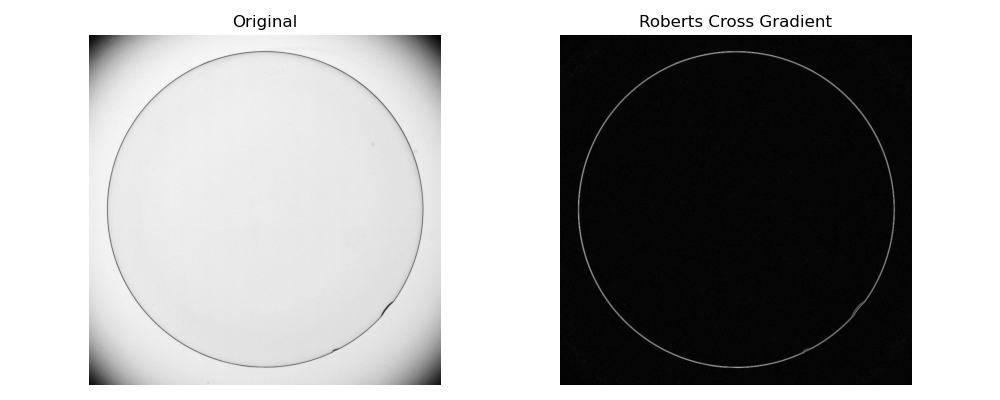
\includegraphics[width=0.8\textwidth]{code/result/p3/roberts_cross_gradient.png}
        \caption{Roberts Cross Gradient Magnitude}
        \label{fig:roberts_cross}
    \end{figure}
    Following is the code used to perform Roberts Cross operator to compute the gradient magnitude.
    \begin{minted}{python}
import os
import cv2 as cv
import numpy as np
import matplotlib
matplotlib.use('Agg')
import matplotlib.pyplot as plt

img = cv.imread('../src/Fig3-1.bmp', cv.IMREAD_GRAYSCALE)
if img is None:
    raise ValueError("Image not found or could not be opened.")
os.makedirs('result/p3', exist_ok=True)

# Roberts mask
Gx = np.array([[1, 0],
               [0, -1]], dtype=np.float32)

Gy = np.array([[0, 1],
               [-1, 0]], dtype=np.float32)

# Convolve with Roberts masks
grad_x = cv.filter2D(img, cv.CV_32F, Gx)
grad_y = cv.filter2D(img, cv.CV_32F, Gy)

# Compute gradient magnitude
grad = cv.magnitude(grad_x, grad_y)
grad = cv.normalize(grad, None, alpha=0, beta=255, norm_type=cv.NORM_MINMAX)
grad = grad.astype(np.uint8)

plt.figure(figsize=(10,4))
plt.subplot(1,2,1)
plt.title('Original')
plt.imshow(img, cmap='gray')
plt.axis('off')

plt.subplot(1,2,2)
plt.title('Roberts Cross Gradient')
plt.imshow(grad, cmap='gray')
plt.axis('off')
plt.tight_layout()
plt.savefig('result/p3/roberts_cross_gradient.png')
    \end{minted}
    \item As Fig.~\ref{fig:enhancement_steps} shows, the results of each step in the image enhancement process.
    \begin{figure}[H]
        \centering
        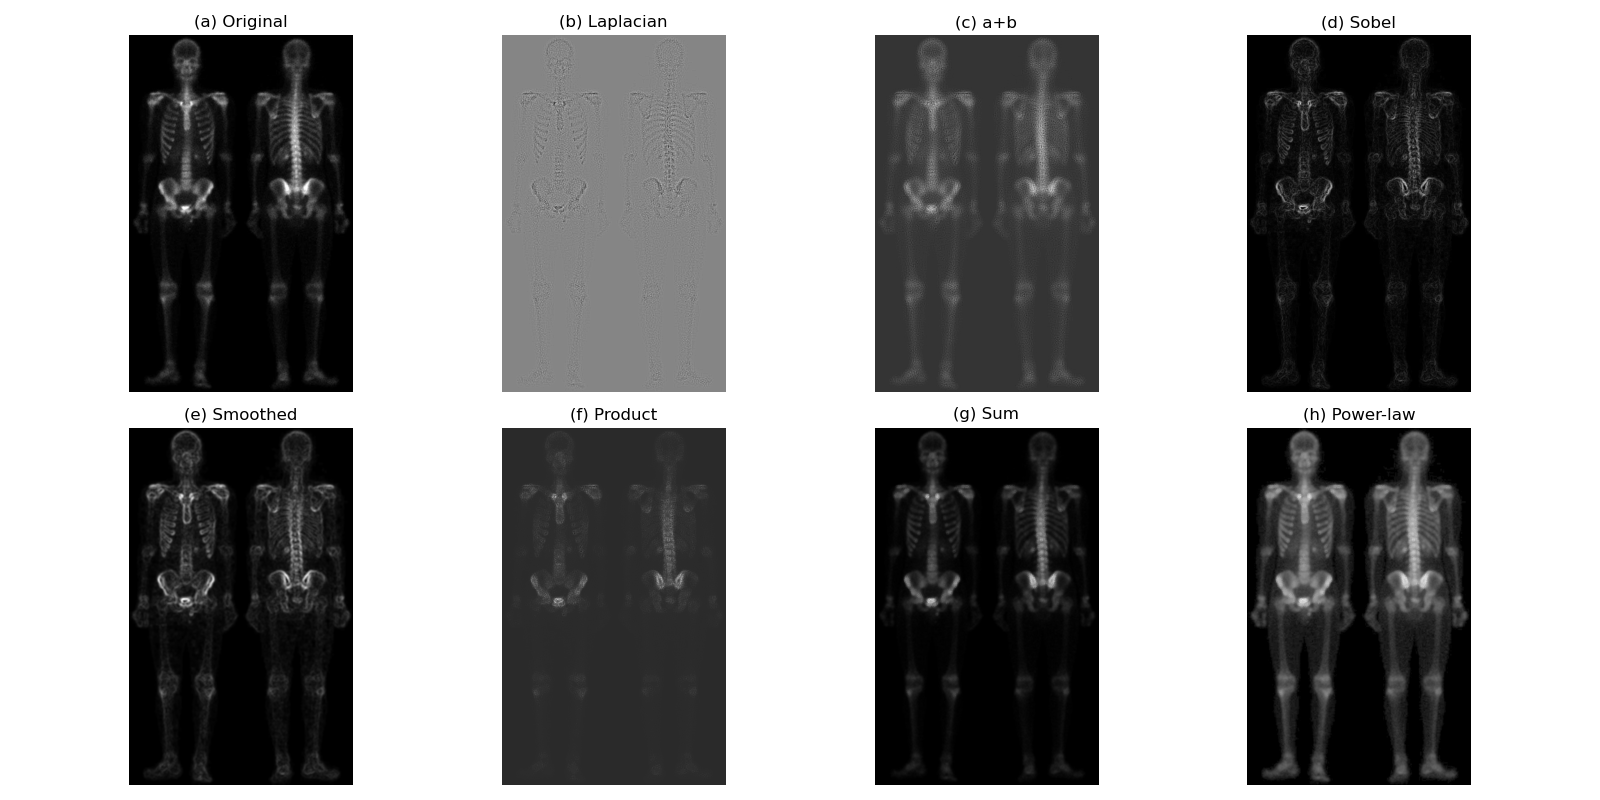
\includegraphics[width=1.0\textwidth]{code/result/p4/enhancement_steps.png}
        \caption{Image Enhancement Steps}
        \label{fig:enhancement_steps}
    \end{figure}
    Following is the code used to perform the image enhancement process.
    \begin{minted}{python}
import os
import cv2 as cv
import numpy as np
import matplotlib
matplotlib.use('Agg')
import matplotlib.pyplot as plt

a = cv.imread('../src/Fig4-1.bmp', cv.IMREAD_GRAYSCALE)
if a is None:
    raise ValueError("Image not found or could not be opened.")
a = a.astype(np.float32)
os.makedirs('result/p4', exist_ok=True)

b = cv.Laplacian(a, cv.CV_32F, ksize=3)

c = cv.add(a, b)

gx = cv.Sobel(a, cv.CV_32F, 1, 0, ksize=3)
gy = cv.Sobel(a, cv.CV_32F, 0, 1, ksize=3)
d = cv.magnitude(gx, gy)

e = cv.blur(d, (5,5))

f = cv.multiply(c, e, scale=1/255.0)

g = cv.add(a, f)

gamma = 0.5
g_norm = cv.normalize(g, None, 0, 1, cv.NORM_MINMAX)
power = np.power(g_norm, gamma)
h = cv.normalize(power, None, 0, 255, cv.NORM_MINMAX).astype(np.uint8)

titles = ['(a) Original', '(b) Laplacian', '(c) a+b', '(d) Sobel',
          '(e) Smoothed', '(f) Product', '(g) Sum', '(h) Power-law']
images = [a, b, c, d, e, f, g, h]

plt.figure(figsize=(16,8))
for i in range(8):
    plt.subplot(2,4,i+1)
    plt.imshow(images[i], cmap='gray')
    plt.title(titles[i])
    plt.axis('off')
plt.tight_layout()
plt.savefig('result/p4/enhancement_steps.png')
    \end{minted}
\end{enumerate}


\end{document}